\section{\MSWaveH{} Algorithm and Analysis}
\label{sec:framework}

In \MSWave{}, we also leverage the multi-resolution property of the
Haar wavelet decomposition of time series. The server $P$ distributes
the reference time series set $Q=\{S_{q1},\ldots,S_{qn}\}$ in a
level-wise manner. That is, $P$ sends the coefficients of each $S_{qi}
\in Q$ to the local machines, one level at a time starting from the
highest level $L$.  At each level, we further prune the candidates,
until the final $k$ answers are found.  While similar to \LeeWave{} at
this high level, \MSWave{} must overcome the limitations outlined in
the prior section.  To do this, first we derive new formulas for
computing the similarity ranges of the three linkage distances between
the reference set and a candidate time series
(Section~\ref{subsec:newbounds}).  These ranges must be effective at
pruning yet guarantee no false dismissals.  Second, we devise a
correct and bandwidth-efficient protocol for the data exchanges
between the server and the multiple local machines
(Section~\ref{subsec:protocol}).  We present two variants:
\MSWave-S{}, which computes the bounds at the server, and \MSWave-L{},
which computes the bounds at the local machines.  Finally, we provide
an analysis of the bandwidth consumption of both variants,
which demonstrates the effectiveness of \MSWave{} at reducing bandwidth
(Section~\ref{subsec:analysis}).

\subsection{Problem Setup}\label{subsec:probset}
There are a query set $Q={\{q_1,q_2,...,q_T\}}\subset\mathbb{R}^D$ at the server $P$ and a dataset $X_i\subset\mathbb{R}^D$ on each local machine $M_i$.  For each query $q_t$, we want to find its $k_{th}$ nearest neighborhood among these distributed datasets while reducing the transmission cost between $P$ and each $M_i$.

\subsection{Orthogonal Transformation}
\newtheorem{Orthogonal}{\bf Definition}
\begin{Orthogonal}
A matrix $W \in\mathbb{R}^{D\times D}$ is orthogonal if whose columns and rows are orthogonal vectors, i.e.
\[
W^{T}W=WW^{T}=I
\]
where $I$ is the identity matrix.
\end{Orthogonal}

\newtheorem{ProOfOrthogonal}{\bf Property}
\begin{ProOfOrthogonal}
Let $x, y\in\mathbb{R}^{D}$, and $W\in\mathbb{R}^{D\times D}$ be an orthogonal matrix. Then,
\[
Dist(x,y)^2=\sum^D_{d=1}{(x[d]-y[d])^2} \\
=\sum^D_{d=1}{(W_dx-W_dy)^2}=Dist(Wx,Wy)^2
\]
where $W_d$ is the $d_{th}$ row of $W$.
\end{ProOfOrthogonal}

\subsection{Computation of Distance Bounds}\label{subsec:newbounds}

We start from the similarity range of the distance between each
individual reference time series $S_{qi}$ to some candidate
$S_x$. Similar to Eq.~\eqref{eq:upper-bound}, we can derive the upper
bound $UB$ and the lower bound $LB$ of $Dst(S_{qi},S_x)$ as soon as all the
coefficients for $S_{qi}$ from the highest level $L$ to the current level
$\ell$ have been sent to the local machines, as follows:

{\small
\begin{eqnarray}
\lefteqn{LB(qi,x) =  accDst^{\ell}(S_{qi},S_{x}).} \label{eq:single-LB} \\
\lefteqn{UB(qi,x) = accDst^{\ell }(S_{qi},S_{x})} \notag \\
& + & \sum_{l=1}^{\ell-1}
 \sum_{p}([n_{(l,p)}^{(qi)}]^{2}+[n_{(l,p)}^{(x)}]^{2}) \times 2^{l} \notag \\
& + & 2 \times \min\{\sqrt{\sum_{l=1}^{\ell-1}\sum_{p}[n_{(l,p)}^{(qi)}
 \times 2^{l}]^{2} \times \sum_{l=1}^{\ell-1}\sum_{p}[n_{(l,p)}^{(x)}]^{2}},
   \notag \\
&&\sqrt{\sum_{l=1}^{\ell-1}\sum_{p}[n_{(l,p)}^{(x)} \times 2^{l}]^{2} \times 
        \sum_{l=1}^{\ell-1}\sum_{p}[n_{(l,p)}^{(qi)}]^{2}}\}.
 \label{eq:single-UB}
\end{eqnarray}
}

Note that Eq.~\eqref{eq:single-UB} is an enhanced version of the upper
bound compared to that in Eq.~\eqref{eq:upper-bound}. Because the
roles of $S_{qi}$ and $S_x$ are interchangeable in the squared terms
in Eq.~\eqref{eq:upper-bound}, a tighter upper bound is obtained by
choosing the minimum among the two choices.  Our experiments will show
that this subtle change noticeably improves the pruning
performance. This new bound does not violate the non-increasing
property proved in \cite{Yeh:2008:LLD} because the smaller bound from
two non-increasing bounds is chosen here.

Now we can derive the similarity range for each linkage distance
defined in Definition~\ref{def:3distances}. For $d_{avg}(Q, S_x)$, 
the average of $Dst(S_{qi},S_x)$ for all $S_{qi} \in Q$, we note that because the
distance is non-negative, we can simply derive the new bounds as
follows.

{\small
\begin{align}
&LB_{avg}(Q, S_x)=\frac{1}{|Q|}\sum_{i=1}^{|Q|}LB(qi, x) \label{eq:avg_LB}\\
&UB_{avg}(Q, S_x)=\frac{1}{|Q|}\sum_{i=1}^{|Q|}UB(qi, x) \label{eq:avg_UB}
\end{align}
}

\noindent
For $d_{sin}(Q, S_x)$, the two bounds are:
{\small
\begin{align}
&LB_{sin}(Q, S_x) = \min_{1 \leq i \leq |Q|}LB(qi, x) 
\label{eq:sin_LB}\\
&UB_{sin}(Q, S_x) = \min_{1 \leq i \leq |Q|}UB(qi, x) \label{eq:sin_UB}
\end{align}
}

\noindent
Finally, for $d_{com}(Q, S_x)$, the two bounds are:
{\small
\begin{align}
&LB_{com}(Q, S_x) = \max_{1 \leq i \leq |Q|}LB(qi, x) \label{eq:com_LB}\\
&UB_{com}(Q, S_x) = \max_{1 \leq i \leq |Q|}UB(qi, x) \label{eq:com_UB}
\end{align}
}

\begin{figure}[tbp]
\subfigure[The upper and lower bounds for $d_{sin}(Q,S_x)$.] {
\label{fig:dsinbound}
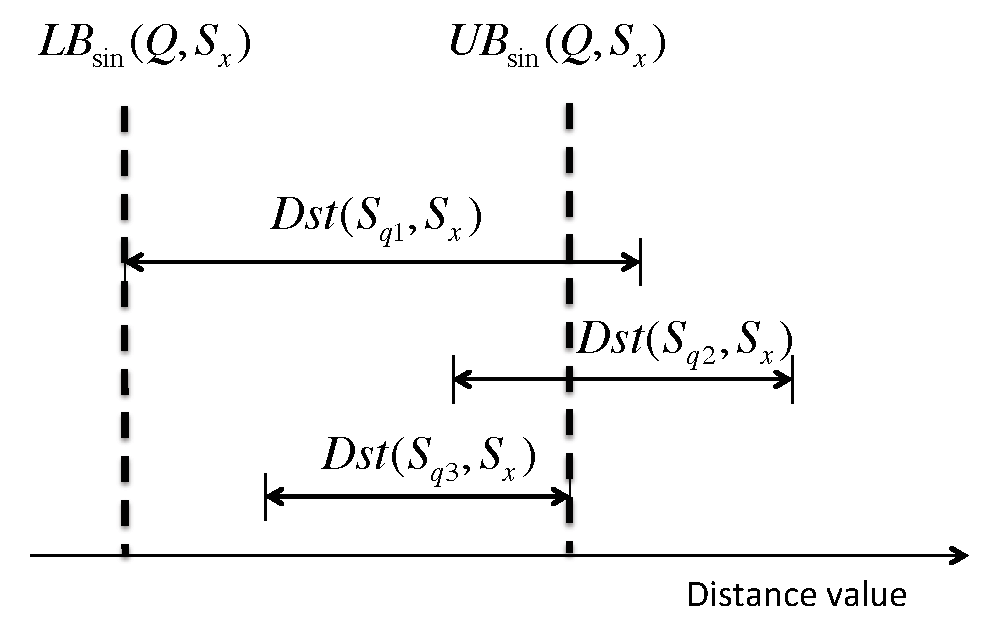
\includegraphics[scale=0.25]{dsinbound.eps}
%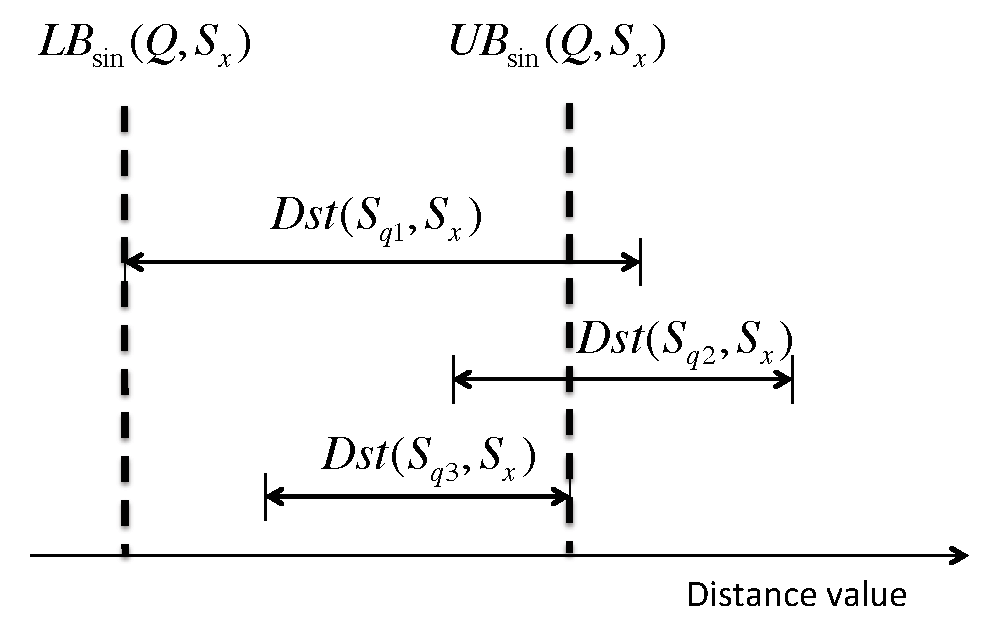
\includegraphics[scale=0.26]{dsinbound.eps}
}
\hspace{0.1cm}
\subfigure[The upper and lower bounds for $d_{com}(Q,S_x)$.] {
\label{fig:dcombound}
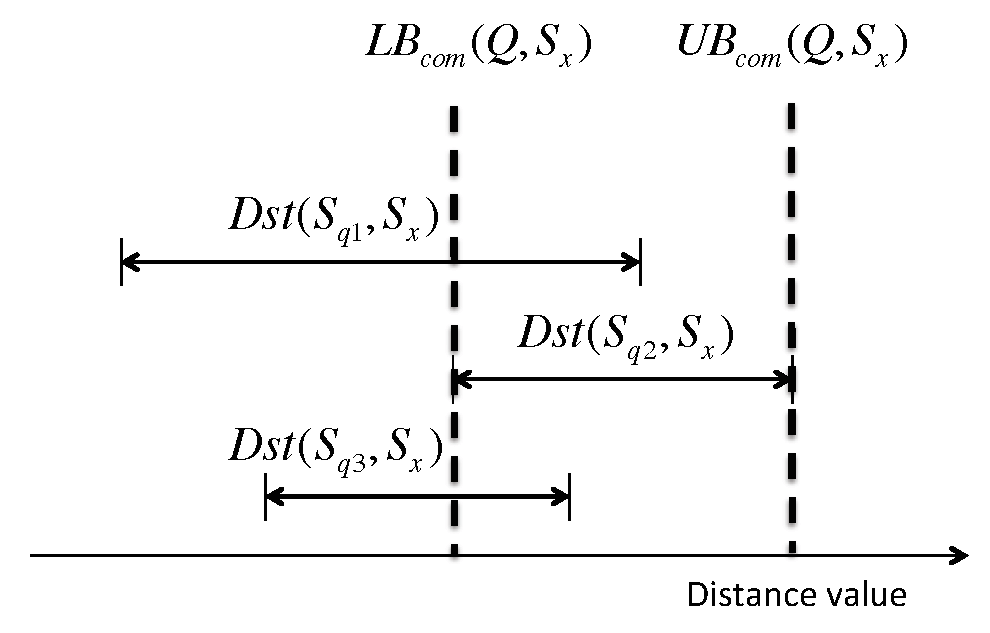
\includegraphics[scale=0.25]{dcombound.eps}
}
\vspace{-0.1in}
\caption{Upper and lower bound computations for different linkage distance measures.}
\label{fig:newbounds}
\vspace{-0.15in}
\end{figure}

Fig.~\ref{fig:dsinbound} illustrates the bounds for $d_{sin}(Q,S_x)$.
As we want to choose the closest distance of
a candidate time series to the reference set $Q$, we can set the lower
(upper) bounds of $d_{sin}(Q,)$ using the smallest ones among all
$LB(qi,x)$ ($UB(qi,x)$, respectively), and for $d_{com}(Q,X)$ using
the largest ones among all $LB(qi,x)$ ($UB(qi,x)$), as shown in
Fig.~\ref{fig:dcombound}.

\begin{figure*}[t!]
\footnotesize
\centering
%\begin{tabular}{|lp{2.95in}|lp{2.95in}|}
\begin{tabular}{|lp{3.2in}|lp{3.2in}|}
\hline
\multicolumn{4}{|p{6in}|}{\textbf{Procedure:} \MSWave-S{} for a $k$NN/$k$FN 
  multiple time series query} \\ 
\multicolumn{4}{|p{6in}|}{\textbf{Input:} $k$, $Q=\{S_{q1},\ldots,S_{qn}\}$, 
  a linkage distance measure (single, average or complete)} \\ 
\multicolumn{4}{|p{6in}|}{\textbf{Output:} The $k$ most similar/dissimilar
  time series to $Q$ according to the designated linkage distance} \\ \hline
\multicolumn{2}{|l|}{\emph{The server $P$:}} & \multicolumn{2}{l|}{\emph{A 
  local machine $M_i$:}} \\
1. & Send coefficients of each $S_{qi} \in Q$ at level $L$ to all  $M$ local 
  machines. & 
2. & For each local candidate time series, $S_x$, compute and return 
  ($Dst^{L}(S_{qi},S_{x})$ $\forall S_{qi} \in Q$, $\sum_{l=1}^{L-1} 
  \sum_{p}[n_{(l,p)}^{(x)}]^{2}$, $\sum_{l=1}^{L-1} 
  \sum_{p}([n_{(l,p)}^{(x)}]^{2}\times 2^l)$, $\sum_{l=1}^{L-1} 
  \sum_{p}([n_{(l,p)}^{(x)}]^{2}\times 2^l)^2$) to $P$. \\ 
3. & Compute the upper and lower bounds based on
  Eq.~\eqref{eq:single-LB}-\eqref{eq:single-UB} for each candidate time series
  to each reference series. Then compute the similarity range for each
  candidate time series to $Q$ according to the designated linkage distance
  based on Eq.~\eqref{eq:avg_LB}-\eqref{eq:com_UB}. Do the first pruning.
  & & \\ 
4. & Repeat steps 5--7 for levels $l=L-1,L-2,\ldots,1$ until \textbf{done}\{
  & & \\ 
5. & Send level coefficients of each $S_{qi} \in Q$ and the ids of any pruned
  candidate series to the appropriate local machines. &
6. & Compute and return a 2-tuple ($Dst^{l}(S_{qi}$, $S_{x})$ $\forall S_{qi}
  \in Q$, $\sum_{p}[n_{(l,p)}^{(x)}]^{2}$) for each local candidate time
  series, $S_x$. \\
7. & Update the upper and lower bounds based on
  Eq.~\eqref{eq:single-LB}-\eqref{eq:single-UB} for each candidate time series
  to each reference series. Then update the bounds of the linkage distance
  based on Eq.~\eqref{eq:avg_LB}-\eqref{eq:com_UB}. Do corresponding pruning
  for $k$NN or $k$FN.  Set \textbf{done} to \textbf{true} if there are
  $k$ candidate time series left. & & \\
8. & \} & & \\
9. & Ask the appropriate machines for the contents
of the final $k$ time series. &
10. & If asked, send back the corresponding full time series contents.\\ \hline
\end{tabular}
\vspace{-0.05in}
\caption{\label{fig:mswave-s}  
Protocol for distributed $k$NN/$k$FN query processing using \MSWave-S{}.}
%\end{figure*}
%
%\begin{figure*}[t]
\vspace{0.15in}
\centering
%\begin{tabular}{|lp{2.95in}|lp{2.95in}|}
\begin{tabular}{|lp{3.2in}|lp{3.2in}|}
\hline
\multicolumn{4}{|p{6in}|}{\textbf{Procedure:} \MSWave-L{} for a $k$NN/$k$FN
  multiple time series query} \\ 
\multicolumn{4}{|p{6in}|}{\textbf{Input:} $k$, $Q=\{S_{q1},\ldots,S_{qn}\}$,
  a linkage distance measure (single, average or complete)} \\ 
\multicolumn{4}{|p{6in}|}{\textbf{Output:} The $k$ most similar/dissimilar time
  series to $Q$ according to the designated linkage distance} \\ \hline
\multicolumn{2}{|l|}{\emph{The server $P$:}} & \multicolumn{2}{l|}{\emph{A
  local machine $M_i$:}} \\
1. & Send level $L$ coefficients,
  $\sum_{l=1}^{L-1} \sum_{p}[n_{(l,p)}^{(qi)}]^2$,
  $\sum_{l=1}^{L-1}\sum_{p}([n_{(l,p)}^{(qi)}]^2 \times 2^{l})$, and
  $\sum_{l=1}^{L-1}\sum_{p}([n_{(l,p)}^{(qi)}]^2 \times 2^{l})^2$
  of each $S_{qi} \in Q$  to all $M$ local machines. & 
2. & For each local candidate time series, $S_x$, compute the individual
  bounds with each reference time series using
  Eq.~\eqref{eq:single-LB}-\eqref{eq:single-UB}. Then compute and return the
  two linkage distances bounds based on
  Eq.~\eqref{eq:avg_LB}-\eqref{eq:com_UB}. \\
3. & Do the first pruning by sorting the upper/lower bounds of each candidate
  series.  & & \\ 
4. & Repeat steps 5--7 for levels $l=L-1,L-2,\ldots,1$ until \textbf{done}\{
  & & \\ 
5. & Send level coefficients of each $S_{qi} \in Q$ and the ids of any pruned
  candidate series to the appropriate local machines. &
6. & Update the corresponding upper/lower bounds based on the computation
  defined in Eq.~\eqref{eq:avg_LB}-\eqref{eq:com_UB} and return the two
  linkage distance bounds for each local candidate time series. \\
7. & Do corresponding pruning for $k$NN or $k$FN according to the updated
  bounds of each candidate series sent back from the local machines.
  Set \textbf{done} to \textbf{true} if there are $k$
  candidate time series left. & & \\
8. & \} & & \\
9. & Ask the appropriate machines for the contents
of the final $k$ time series. &
10. & If asked, send back the corresponding full time series contents.\\ \hline
\end{tabular}
\vspace{-0.05in}
\caption{\label{fig:mswave-l}
Protocol for distributed $k$NN/$k$FN query processing using \MSWave-L{}.}
\end{figure*}

Now we prove the similarity ranges bounded by these lower and upper
bounds will shrink as more levels of coefficients are disseminated to
local machines.

\begin{theorem} \label{theo:avg-bound-shrink}
$UB_{avg}(Q, S_x)$ is non-increasing and $LB_{avg}(Q, S_x)$ is
non-decreasing when the coefficients of $S_{qi} \in Q$ are
disseminated from level $\ell$ to level $\ell-1$
\end{theorem}

\textbf{Proof:} As argued above, it readily follows from
\cite{Yeh:2008:LLD} that Eq.~\eqref{eq:single-LB} is non-decreasing
and Eq.~\eqref{eq:single-UB} is non-increasing. Therefore,
$LB_{avg}(Q, S_x)$ must be non-decreasing and $UB_{avg}(Q, S_x)$ must
be non-increasing as they are each just the average of a set of such
non-decreasing and non-increasing bounds.  \hfill $\blacksquare$

\begin{theorem} \label{theo:sin-bound-shrink}
$UB_{sin}(Q, S_x)$ is non-increasing and $LB_{sin}(Q, S_x)$ is
non-decreasing when the coefficients of $S_{qi} \in Q$ are
disseminated from level $\ell$ to level $\ell-1$
\end{theorem}

\textbf{Proof:} Let $l(\ell)$ and $u(\ell)$ be the reference time
series in $Q$ that have the smallest lower bound and smallest upper
bound of the similarity range to $S_x$ at level $\ell$. That is,

{\small
\begin{eqnarray*}
l(\ell)& = & \arg\min_{1\leq i \leq |Q|}LB(qi,x)|_{\ell}
\hspace{0.3in} \textrm{and}\\
u(\ell)& = & \arg\min_{1\leq i \leq |Q|}UB(qi,x)|_{\ell},
\end{eqnarray*}
}

\noindent
where $|_{\ell}$ represents the corresponding bound values are 
derived at level $\ell$. We have
{\small
\begin{eqnarray*}
\lefteqn{LB_{sin}(Q,S_x)|_\ell = LB(q_{l(\ell)},x)|_\ell 
 \leq LB(q_{l(\ell-1)},x)|_\ell} \\
 &&\leq LB(q_{l(\ell-1)},x)|_{\ell-1} = LB_{sin}(Q,S_x|_{\ell-1}),
\end{eqnarray*}}

\noindent
where the first inequality holds because $l(\ell)$ is the arg min at
level $\ell$ and the second inequality holds because
Eq.~\eqref{eq:single-LB} is non-decreasing.  Thus, $LB_{sin}(Q,S_x)$ is
non-decreasing.

Similarly, because Eq.~\eqref{eq:single-UB} is non-increasing, a symmetric
argument shows that $UB_{sin}(Q,S_x)$ is non-increasing.
\hfill $\blacksquare$

Finally, the symmetry between the bounds for $d_{syn}$ and $d_{com}$
yields the following.
\begin{theorem}
\label{theo:com-bound-shrink}
$UB_{com}(Q, S_x)$ is non-increasing and $LB_{com}(Q, S_x)$ is
non-decreasing when the coefficients of $S_{qi} \in Q$ are
disseminated from level $\ell$ to level $\ell-1$.
\end{theorem}

\vspace{-0.1in}
\subsection{The \MSWave{} Protocol}\label{subsec:protocol}

We are now ready to describe the details of how \MSWave{} processes a
distributed $k$NN or $k$FN multiple time series query in a level-wise
manner and how the server $P$ progressively prunes the candidates. 
We will present two schemes to solve this problem: \MSWave-S{} and \MSWave-L{}. 

\textbf{\MSWave-S{}: Server computes the bounds.}
Fig.~\ref{fig:mswave-s} presents the \MSWave-S{} protocol. At the
initial step, the server $P$ sends the highest level-$L$ coefficients
of each $S_{qi}$ in $Q$ to all $M$ local machines. Each local machine
then extracts wavelet coefficients of the same level for each time
series to be matched.  It then returns the following numbers for each
local candidate time series $S_x$: the level-$L$ distance,
$Dst^{L}(S_{qi}, S_x)$, for $i=1$ to $|Q|$, and three other numbers that
will be used by $P$ to generate the bounds for pruning:
{\small
%\[
$\sum_{l=1}^{L-1}\sum_{p}[n_{(l,p)}^{(x)}]^2$,
$\sum_{l=1}^{L-1}\sum_{p}([n_{(l,p)}^{(x)}]^2 \times 2^{l})$
% \hspace{0.1in}
\textrm{and}
% \hspace{0.1in} 
$\sum_{l=1}^{L-1}\sum_{p}([n_{(l,p)}^{(x)}]^2 \times 2^{l})^2$.
%\]
}
%
%\noindent
After receiving these numbers from each candidate time series, $P$
updates the lower and upper bounds based on Eq.~\eqref{eq:single-LB}
and Eq.~\eqref{eq:single-UB} for each candidate time series.

It then does some initial pruning to remove any candidates that
cannot be among the top $k$ neighbors. To prune candidates for $k$NN
queries, $P$ first sorts the candidate time series in an ascending
order based on the upper bounds.  Any candidate time series whose
similarity lower bound is higher than the upper bound of the $k^{th}$
time series in the sorted list cannot be in the final answer, and thus
is pruned.  As the bound is proved to be monotonically non-increasing
from level to level, we can guarantee that there are no false
dismissals under this pruning strategy. Similarly, for $k$FN query, any
candidate time series whose similarity upper bound is smaller than the
$k^{th}$ largest lower bound cannot be in the final answer. Then, $P$
moves to the next level.

For any given level $l$, $P$ sends the level-$l$ coefficients of each
$S_{qi} \in Q$ and the ids of any pruned time series to the appropriate local
machines.  The local machine returns two level-specific numbers
for each (remaining) candidate time series: $Dst^{l}(S_{qi}, S_x)$ for $i=1$ to
$|Q|$ and $\sum_{p}[n_{(l,p)}^{(x)}]^2$.  $P$ then uses these values to
update the upper/lower bounds, always making them tighter. With the
bounds of each candidate series to each reference time series, $P$
further computes the similarity range under the prespecified linkage distance
of each series to the reference set $Q$ based on
Eq.~\eqref{eq:avg_LB}--\eqref{eq:com_UB}. With increasingly tighter
ranges, $P$ can better prune the candidate list.  The algorithm ends
when there are $k$ candidate time series remaining.

\textbf{\MSWave-L{}: Local machines compute the bounds.}
Note that with \MSWave-S{}, the local machines consume
bandwidth to send back the level distances of each time series to
multiple reference time series, i.e., $Dst^{l}(S_{qi}, S_x)$ for $i=1$
to $|Q|$, which grows linearly with Q. When $|Q|$ becomes large, the
\MSWave-S{} protocol might not be as efficient.

To deal with this issue, we propose another scheme, \MSWave-L{},
which computes the similarity bounds under the linkage distance at the
local machines. By doing so, we need not send the level distances for
each reference time series, but instead only 2 single bound values for
the whole query set, reducing bandwidth.

Fig.~\ref{fig:mswave-l} presents the protocol. In the initial step,
the server $P$ sends to the local machines not only the coefficients
at level $L$, but also three additional numbers for each reference time
series $S_{qi} \in Q$, which will later enable the local machines to
generate the similarity ranges:
{\small
%\[
$\sum_{l=1}^{L-1}\sum_{p}[n_{(l,p)}^{(qi)}]^2$,
$\sum_{l=1}^{L-1}\sum_{p}([n_{(l,p)}^{(qi)}]^2 \times 2^{l})$
% \hspace{0.1in}
\textrm{and}
% \hspace{0.1in} 
$\sum_{l=1}^{L-1}\sum_{p}([n_{(l,p)}^{(qi)}]^2 \times 2^{l})^2$.
%\]
}
%
%\noindent
After receiving these values, the local machines can compute the
similarity bounds of each candidate series to $Q$ based on
Eq.~\eqref{eq:avg_LB}--\eqref{eq:com_UB} according to different linkage
distance measures. Then, each local machine sends back only the two bound
values for each candidate series to the server. With the bounds of
each candidate, the server $P$ can then do corresponding pruning to
tell the local machines which candidates cannot be in the final $k$
results and can be discarded. This procedure proceeds iteratively until the
final results are produced. Note that the pruning strategy is the same
as that done in \MSWave-S{}.


\vspace{-0.1in}
\subsection{Analysis of Bandwidth Consumption}\label{subsec:analysis}

We will now analyze the bandwidth consumption of \MSWave-L{} relative to
\MSWave-S{}. Suppose there are a total of $s$ time series distributed in
$m$ local machines, and $|Q|$ reference time series.
%, and the length of each time series is $T$. For simplicity of exposition, assume $T$ is a power of 2.
%By Haar wavelet decomposition, there will be
%$L=\log_2{T}$ levels of wavelet coefficients for each time series, and
%there are $2^{L-\ell+1}$ number of coefficients at some level $\ell$. 
Let $s_{\ell}$ be the number of candidate time series remaining at
level $\ell$.  We have that the difference in bandwidth between 
\MSWave-S{} and \MSWave-L{} is:
$-3|Q|m + s(4|Q|-2) + \sum_{\ell}{ 2s_{\ell}(|Q|-1) }$, which equals
{\small
\begin{equation}
|Q|( 4s -3m +2\sum_{\ell}{s_{\ell}} ) -2s - 2\sum_{\ell}{s_{\ell}}.
 \label{eq:bandwidthsaved}
\end{equation}
}

\noindent
The term $-3|Q|m$ refers to the three more summation values
sent by $P$ to local machines in step 1 in \MSWave-L{}. The term
$s(4|Q|-2)$ is the bandwidth saved by transmitting only the 2 bounds
for each $\{Q, S_x\}$ instead of all pair-wise reference-candidate
level distances and the related summation values in step 2. The final
summation term describes the bandwidth saved at the following steps
when more and more levels of coefficients are disseminated.

Note that Eq.~\eqref{eq:bandwidthsaved} is always
greater than zero.  Because in general cases $s \geq m$ (otherwise the
data do not have to be distributed to $m$ machines), we have
$|Q|(4s-3m)-2s>(|Q|-2)s \geq 0$, because $|Q|>1$ for multiple
time series, and the final term $2s(|Q|-1)$ is also greater than zero.
Moreover, \MSWave-L{}'s bandwidth savings over \MSWave-S{} increases
linearly with $|Q|$.

%Consequently, the bandwidth consumption for \MSWave-S{} is

%{\footnotesize
%\begin{align}
%&|Q|*M*2 + |Q|*N*4 + N + \notag\\
%&\sum_{\ell}{(|Q|*M_{\ell}*2^{L-\ell+1} + |Q|*N_{\ell}*2+N_{\ell})},
%\label{eq:cost_of_mswave-s}
%\end{align}
%}
%and for \MSWave-L{} is
%{\footnotesize
%\begin{align}
%& |Q|*M*(2+3) + N*(2+1) + \notag\\
%& \sum_{\ell}{(|Q|*M_{\ell}*2^{L-\ell+1} + N_{\ell}*(2+1))},
%\label{eq:cost_of_mswave-l}
%\end{align}
%}
%where $M_{\ell}$ and $N_{\ell}$ is the number of machines having candidate time series and the number of candidate time series left at level $\ell$.

%By subtracting Eq.~\eqref{eq:cost_of_mswave-s} from Eq.~\eqref{eq:cost_of_mswave-l} we have the bandwidth saved by \MSWave-L{} compared to \MSWave-S{} as follows.
